\begingroup
\begin{figure}[!htb]
    % \setArraystrech{1.5}
    \setlength\tabcolsep{1pt}
    \centering
    \begin{tabular*}{0.85\textwidth}{ c c c c c c }
        & Target & Output & Normal & Depth & Voxel \\
        %%%%%%%%%%%%%%%%%%%
        %%%%% GUITARS %%%%%
        %%%%%%%%%%%%%%%%%%%

        %%%%% GUITARS_EXVA %%%%%
        ExVA &
        \setlength\tabcolsep{0pt}
        \begin{tabular}{cc}
            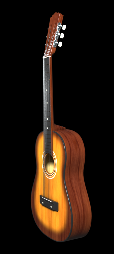
\includegraphics[width=0.07\textwidth]{figures/results/stat_set/valid/guitar4_targ_256px.png} & 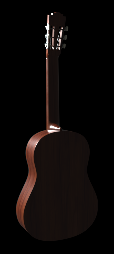
\includegraphics[width=0.07\textwidth]{figures/results/stat_set/valid/guitar8_targ_256px.png}
        \end{tabular}
        &
        \setlength\tabcolsep{0pt}
        \begin{tabular}{cc}
            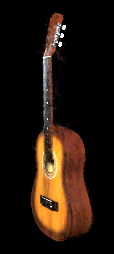
\includegraphics[width=0.07\textwidth]{figures/results/stat_set/valid/guitar4_exva_89k.png} & 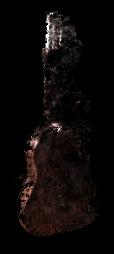
\includegraphics[width=0.07\textwidth]{figures/results/stat_set/valid/guitar8_exva_89k.png}
        \end{tabular}
        &
        \setlength\tabcolsep{0pt}
        \begin{tabular}{cc}
            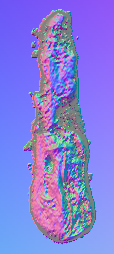
\includegraphics[width=0.07\textwidth]{figures/results/stat_set/valid/guitar4_exva_normal_89k.png} & 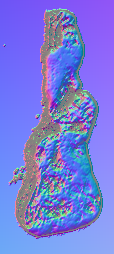
\includegraphics[width=0.07\textwidth]{figures/results/stat_set/valid/guitar8_exva_normal_89k.png}
        \end{tabular}
        &
        \setlength\tabcolsep{0pt}
        \begin{tabular}{cc}
            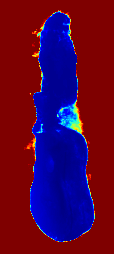
\includegraphics[width=0.07\textwidth]{figures/results/stat_set/valid/guitar4_exva_depth_89k.png} & 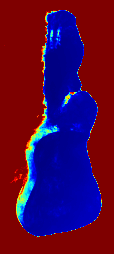
\includegraphics[width=0.07\textwidth]{figures/results/stat_set/valid/guitar8_exva_depth_89k.png}
        \end{tabular}
        &
        \setlength\tabcolsep{0pt}
        \begin{tabular}{cc}
            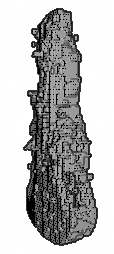
\includegraphics[width=0.07\textwidth]{figures/results/stat_set/valid/guitar4_exva_voxel_89k.png} & 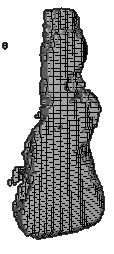
\includegraphics[width=0.07\textwidth]{figures/results/stat_set/valid/guitar8_exva_voxel_89k.png}
        \end{tabular} \\[-5pt]

        %%%%% GUITARS_NSVF %%%%%
        NSVF &
        \setlength\tabcolsep{0pt}
        \begin{tabular}{cc}
            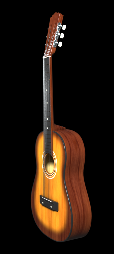
\includegraphics[width=0.07\textwidth]{figures/results/stat_set/valid/guitar4_targ_256px.png} & 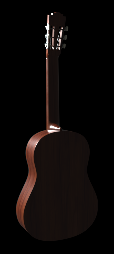
\includegraphics[width=0.07\textwidth]{figures/results/stat_set/valid/guitar8_targ_256px.png}
        \end{tabular}
        &
        \setlength\tabcolsep{0pt}
        \begin{tabular}{cc}
            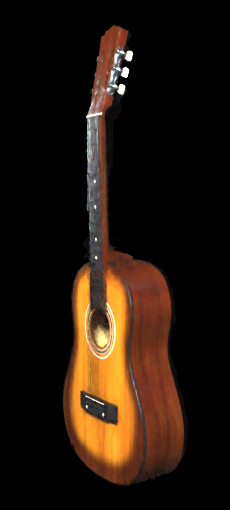
\includegraphics[width=0.07\textwidth]{figures/results/stat_set/valid/guitar4_nsvf_119k.png} & 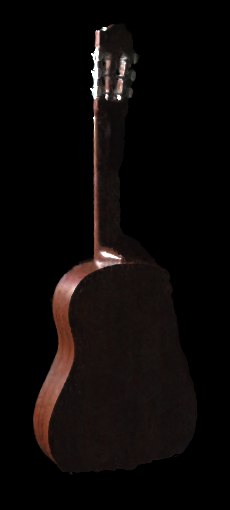
\includegraphics[width=0.07\textwidth]{figures/results/stat_set/valid/guitar8_nsvf_119k.png}
        \end{tabular}
        &
        \setlength\tabcolsep{0pt}
        \begin{tabular}{cc}
            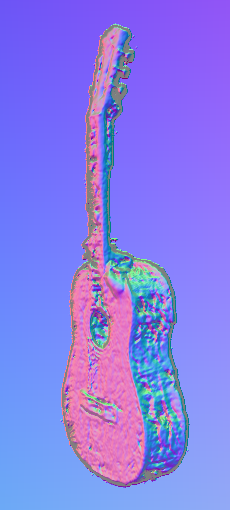
\includegraphics[width=0.07\textwidth]{figures/results/stat_set/valid/guitar4_nsvf_normal_119k.png} & 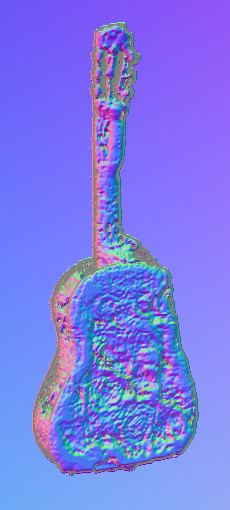
\includegraphics[width=0.07\textwidth]{figures/results/stat_set/valid/guitar8_nsvf_normal_119k.png}
        \end{tabular}
        &
        \setlength\tabcolsep{0pt}
        \begin{tabular}{cc}
            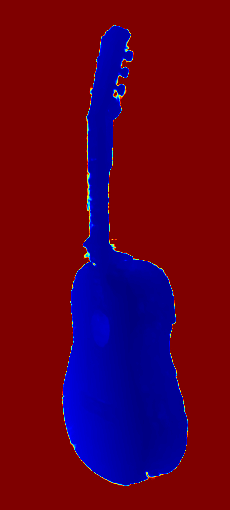
\includegraphics[width=0.07\textwidth]{figures/results/stat_set/valid/guitar4_nsvf_depth_119k.png} & 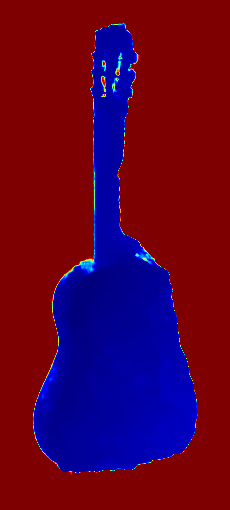
\includegraphics[width=0.07\textwidth]{figures/results/stat_set/valid/guitar8_nsvf_depth_119k.png}
        \end{tabular}
        &
        \setlength\tabcolsep{0pt}
        \begin{tabular}{cc}
            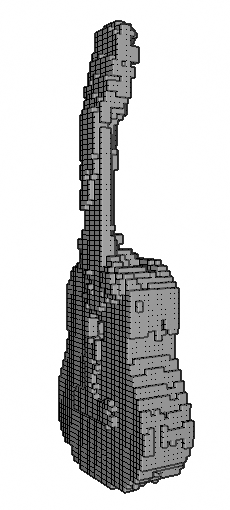
\includegraphics[width=0.07\textwidth]{figures/results/stat_set/valid/guitar4_nsvf_voxel_119k.png} & 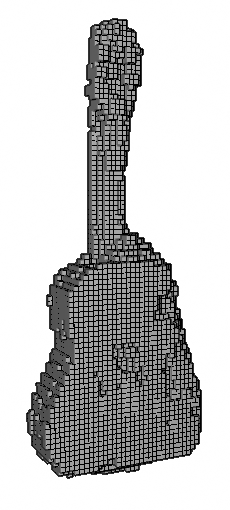
\includegraphics[width=0.07\textwidth]{figures/results/stat_set/valid/guitar8_nsvf_voxel_119k.png}
        \end{tabular} \\[0pt]
        
        %%%%%%%%%%%%%%%%%%%
        %%%%% HOTDOGS %%%%%
        %%%%%%%%%%%%%%%%%%%
        
        %%%%% HOTDOG_EXVA %%%%%
        ExVA &
        \begin{tabular}{cc}
            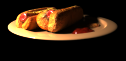
\includegraphics[width=0.14\textwidth]{figures/results/stat_set/valid/hotdog8_targ_128px.png} \\[-6pt]
            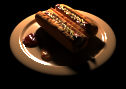
\includegraphics[width=0.14\textwidth]{figures/results/stat_set/valid/hotdog10_targ_128px.png}
        \end{tabular}
        &
        \begin{tabular}{cc}
            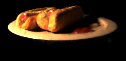
\includegraphics[width=0.14\textwidth]{figures/results/stat_set/valid/hotdog8_exva_55k.png} \\[-6pt]
            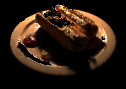
\includegraphics[width=0.14\textwidth]{figures/results/stat_set/valid/hotdog10_exva_55k.png}
        \end{tabular}
        &
        \begin{tabular}{cc}
            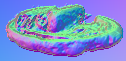
\includegraphics[width=0.14\textwidth]{figures/results/stat_set/valid/hotdog8_exva_normal_55k.png} \\[-6pt]
            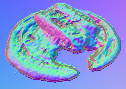
\includegraphics[width=0.14\textwidth]{figures/results/stat_set/valid/hotdog10_exva_normal_55k.png}
        \end{tabular}
        &
        \begin{tabular}{cc}
            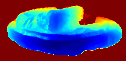
\includegraphics[width=0.14\textwidth]{figures/results/stat_set/valid/hotdog8_exva_depth_55k.png} \\[-6pt]
            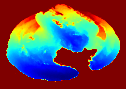
\includegraphics[width=0.14\textwidth]{figures/results/stat_set/valid/hotdog10_exva_depth_55k.png}
        \end{tabular}
        &
        \begin{tabular}{cc}
            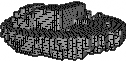
\includegraphics[width=0.14\textwidth]{figures/results/stat_set/valid/hotdog8_exva_voxel_55k.png} \\[-6pt]
            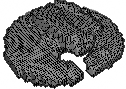
\includegraphics[width=0.14\textwidth]{figures/results/stat_set/valid/hotdog10_exva_voxel_55k.png}
        \end{tabular} \\[-5pt]
        
        %%%%% HOTDOG_NSVF %%%%%
        NSVF &
        \begin{tabular}{cc}
            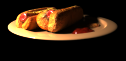
\includegraphics[width=0.14\textwidth]{figures/results/stat_set/valid/hotdog8_targ_128px.png} \\[-6pt]
            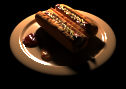
\includegraphics[width=0.14\textwidth]{figures/results/stat_set/valid/hotdog10_targ_128px.png}
        \end{tabular}
        &
        \begin{tabular}{cc}
            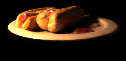
\includegraphics[width=0.14\textwidth]{figures/results/stat_set/valid/hotdog8_nsvf_57k.png} \\[-6pt]
            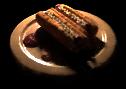
\includegraphics[width=0.14\textwidth]{figures/results/stat_set/valid/hotdog10_nsvf_57k.png}
        \end{tabular}
        &
        \begin{tabular}{cc}
            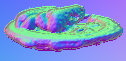
\includegraphics[width=0.14\textwidth]{figures/results/stat_set/valid/hotdog8_nsvf_normal_57k.png} \\[-6pt]
            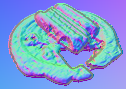
\includegraphics[width=0.14\textwidth]{figures/results/stat_set/valid/hotdog10_nsvf_normal_57k.png}
        \end{tabular}
        &
        \begin{tabular}{cc}
            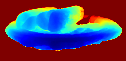
\includegraphics[width=0.14\textwidth]{figures/results/stat_set/valid/hotdog8_nsvf_depth_57k.png} \\[-6pt]
            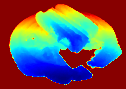
\includegraphics[width=0.14\textwidth]{figures/results/stat_set/valid/hotdog10_nsvf_depth_57k.png}
        \end{tabular}
        &
        \begin{tabular}{cc}
            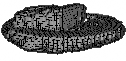
\includegraphics[width=0.14\textwidth]{figures/results/stat_set/valid/hotdog8_nsvf_voxel_57k.png} \\[-6pt]
            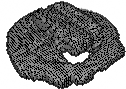
\includegraphics[width=0.14\textwidth]{figures/results/stat_set/valid/hotdog10_nsvf_voxel_57k.png}
        \end{tabular} \\[0pt]
        
        %%%%%%%%%%%%%%%%%%%
        %%%%% LEGOS %%%%%
        %%%%%%%%%%%%%%%%%%%
        
        %%%%% LEGO_EXVA %%%%%
        ExVA &
        \begin{tabular}{cc}
            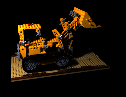
\includegraphics[width=0.14\textwidth]{figures/results/stat_set/valid/lego0_targ_128px.png} \\[-6pt]
            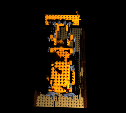
\includegraphics[width=0.14\textwidth]{figures/results/stat_set/valid/lego2_targ_128px.png}
        \end{tabular}
        &
        \begin{tabular}{cc}
            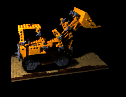
\includegraphics[width=0.14\textwidth]{figures/results/stat_set/valid/lego0_exva_55k.png} \\[-6pt]
            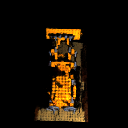
\includegraphics[width=0.14\textwidth]{figures/results/stat_set/valid/lego2_exva_55k.png}
        \end{tabular}
        &
        \begin{tabular}{cc}
            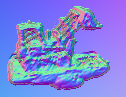
\includegraphics[width=0.14\textwidth]{figures/results/stat_set/valid/lego0_exva_normal_55k.png} \\[-6pt]
            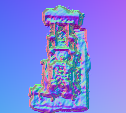
\includegraphics[width=0.14\textwidth]{figures/results/stat_set/valid/lego2_exva_normal_55k.png}
        \end{tabular}
        &
        \begin{tabular}{cc}
            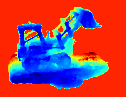
\includegraphics[width=0.14\textwidth]{figures/results/stat_set/valid/lego0_exva_depth_55k.png} \\[-6pt]
            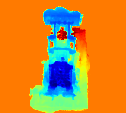
\includegraphics[width=0.14\textwidth]{figures/results/stat_set/valid/lego2_exva_depth_55k.png}
        \end{tabular}
        &
        \begin{tabular}{cc}
            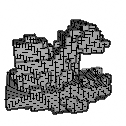
\includegraphics[width=0.14\textwidth]{figures/results/stat_set/valid/lego0_exva_voxel_55k.png} \\[-6pt]
            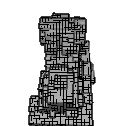
\includegraphics[width=0.14\textwidth]{figures/results/stat_set/valid/lego2_exva_voxel_55k.png}
        \end{tabular} \\[-5pt]
        
        %%%%% LEGO_NSVF %%%%%
        NSVF &
        \begin{tabular}{cc}
            \includegraphics[width=0.14\textwidth]{figures/results/stat_set/valid/lego0_targ_128px.png} \\[-6pt]
            \includegraphics[width=0.14\textwidth]{figures/results/stat_set/valid/lego2_targ_128px.png}
        \end{tabular}
        &
        \begin{tabular}{cc}
            \includegraphics[width=0.14\textwidth]{figures/results/stat_set/valid/lego0_nsvf_57k.png} \\[-6pt]
            \includegraphics[width=0.14\textwidth]{figures/results/stat_set/valid/lego2_nsvf_57k.png}
        \end{tabular}
        &
        \begin{tabular}{cc}
            \includegraphics[width=0.14\textwidth]{figures/results/stat_set/valid/lego0_nsvf_normal_57k.png} \\[-6pt]
            \includegraphics[width=0.14\textwidth]{figures/results/stat_set/valid/lego2_nsvf_normal_57k.png}
        \end{tabular}
        &
        \begin{tabular}{cc}
            \includegraphics[width=0.14\textwidth]{figures/results/stat_set/valid/lego0_nsvf_depth_57k.png} \\[-6pt]
            \includegraphics[width=0.14\textwidth]{figures/results/stat_set/valid/lego2_nsvf_depth_57k.png}
        \end{tabular}
        &
        \begin{tabular}{cc}
            \includegraphics[width=0.14\textwidth]{figures/results/stat_set/valid/lego0_nsvf_voxel_57k.png} \\[-6pt]
            \includegraphics[width=0.14\textwidth]{figures/results/stat_set/valid/lego2_nsvf_voxel_57k.png}
        \end{tabular}
        

    \end{tabular*}
    \caption{The overview of some novel view synthesis results
    achieved with \textit{ExVA} and \textit{NSVF} methods trained on static light setting datasets.
    Each row correspond to a dataset, each subrow shows outputs of the corresponding method.
    Columns correspond to the output maps.
    Note how both schemes fail to learn geometry in the shadowed regions.
    It can also be seen how more the \textit{ExVA} method is sensitive
    to inconsistent geometry comparing with the \textit{NSVF} renders.
    \im{REVIEW: add ImNF results, restructure table:
    ((ExVA:targ1|out1|norm1|vox1||targ2|out2|norm2|vox2 (newline)
    ExNSVF:targ1|out1|norm1|vox1||targ2|out2|norm2|vox2 (newline)
    ImNF:targ1|out1|norm1|vox1||targ2|out2|norm2|vox2))}
    }
    
    \im{static results for ImNF: lego256 u4110, hotdog256 u4109, guitar256 u4105}
    \label{fig:static_valid_results}
\end{figure}
\endgroup